% A0 portrait research poster built on the repository's btrpstr template.
% Build: powershell -ExecutionPolicy Bypass -File scripts/build_poster.ps1
\documentclass[a0v]{btrpstr}
\usepackage{lmodern}
\usepackage{fontspec}
\setmainfont{FiraSans-Regular.otf}[BoldFont=FiraSans-Bold.otf,
 ItalicFont=FiraSans-Italic.otf,BoldItalicFont=FiraSans-BoldItalic.otf]
\usepackage{amsmath,amssymb,graphicx,booktabs,qrcode}
\errorcontextlines=50
\usepackage[hidelinks]{hyperref}
\usetikzlibrary{positioning}
\definecolor{navy}{HTML}{152D43}
\definecolor{teal}{HTML}{087F8C}
\definecolor{orange}{HTML}{E78335}
\definecolor{paper}{HTML}{F3F6F8}
\definecolor{muted}{HTML}{536B7D}
\newcommand{\bodyfont}{\fontsize{29}{37}\selectfont\raggedright}
\newcommand{\smallfont}{\fontsize{26}{33}\selectfont}
\newcommand{\captionfont}{\fontsize{23}{29.5}\selectfont\color{muted}}
\newcommand{\postersectionfont}{\fontsize{37}{45}\selectfont\bfseries}
\newcommand{\subhead}[1]{\par\vspace{.45cm}{\bfseries\color{teal}#1}\par\vspace{.15cm}}
\newcommand{\sourcecaption}[1]{{\captionfont #1\par}}
\newcommand{\setuprow}[2]{\textbf{#1}\enspace #2\par\vspace{.18cm}}
\hypersetup{pdftitle={RACE: Scalable Statistical Estimation of Functional Consistency in LLM Neurons},
 pdfauthor={Runyu Wang, Bo Liu, Xiaxin Zhang, Yu Han, Jiawei Cao, Xiaoye Zhang, Zhe Zhang, Yifan Yang, Peng Ping}}
\begin{document}
\begin{poster}[fontsizes=28pt]
\color{navy}
\posterbackground{fill=paper}
\path[fill=teal] (poster.north west) rectangle ([yshift=-.55cm]poster.north east);
\newpostercol{title}{start={([xshift=2cm,yshift=-.9cm]poster.north west)},width=80.1cm}
\begin{posterbox}{titlebox}{col=title,sep=0pt}
\centering
\begin{minipage}[c]{45.5cm}\centering
{\fontsize{64}{72}\selectfont\bfseries
RACE: Scalable Statistical Estimation\\
of Functional Consistency in LLM Neurons\par}
\vspace{.7cm}
{\fontsize{36}{46}\selectfont
Runyu Wang\textsuperscript{1}, Bo Liu\textsuperscript{2}, Xiaxin Zhang\textsuperscript{1}, Yu Han\textsuperscript{1}, Jiawei Cao\textsuperscript{1},\\
Xiaoye Zhang\textsuperscript{3}, Zhe Zhang\textsuperscript{4}, Yifan Yang\textsuperscript{4}, Peng Ping\textsuperscript{1,*}\par}
\vspace{.45cm}
{\fontsize{29}{37}\selectfont\color{muted}
\textsuperscript{1}Nantong University\quad
\textsuperscript{2}Chongqing University of Post and Telecommunications\\
\textsuperscript{3}China Southern Power Grid Company Limited\quad \textsuperscript{4}Meituan\par}
\end{minipage}
\par
\end{posterbox}
% Logos sit in absolutely positioned nodes so the title stays geometrically centered.
\node[anchor=west] at ([xshift=1cm]titlebox.west)
 {
\includegraphics[width=16cm]{assets/logo/emnlp_2026_logo_v1.png}};
\node[anchor=east] at ([xshift=-1cm]titlebox.east)
 {\begin{minipage}[c]{10.8cm}\centering
 
\includegraphics[width=10.8cm]{assets/logo/ntu_logo.pdf}\\[.35cm]
 
\includegraphics[width=10.8cm]{assets/logo/cqupt.pdf}\\[.35cm]
 
\includegraphics[width=10.8cm]{assets/logo/csg.pdf}\\[.35cm]
 
\includegraphics[width=10.8cm]{assets/logo/meituan.pdf}
 \end{minipage}};
% A dominant full-width finding follows the vertical betterposter template.
\path[fill=navy] ([yshift=-13.5cm]poster.north west) rectangle ([yshift=-24.1cm]poster.north east);
\node[anchor=north west,inner sep=0pt,text width=77cm,text=white]
 (leader) at ([xshift=3.55cm,yshift=-14.15cm]poster.north west) {
 {\fontsize{84}{91}\selectfont
 \textbf{Stable residual alignment}\\
 reveals neurons for\\
 \textbf{specific model behaviors.}\par}
};
\newpostercol{method1}{start={([xshift=2cm,yshift=-25.3cm]poster.north west)},width=39.15cm}
\newpostercol{method2}{start={([xshift=42.95cm,yshift=-25.3cm]poster.north west)},width=39.15cm}
\begin{headerbox}{rda}{col=method1,header={01\quad Collect Signed Evidence},header font=\postersectionfont,
 header style={fill=teal,text=white},body style={fill=white},sep=.65cm,font=\bodyfont}
Strong activations alone can hide inconsistent behavior. RDA collects signed residual evidence across all generated tokens (code/math) or teacher-forced tokens (reference/PyComp-1K).
\vspace{.4cm}
\begin{center}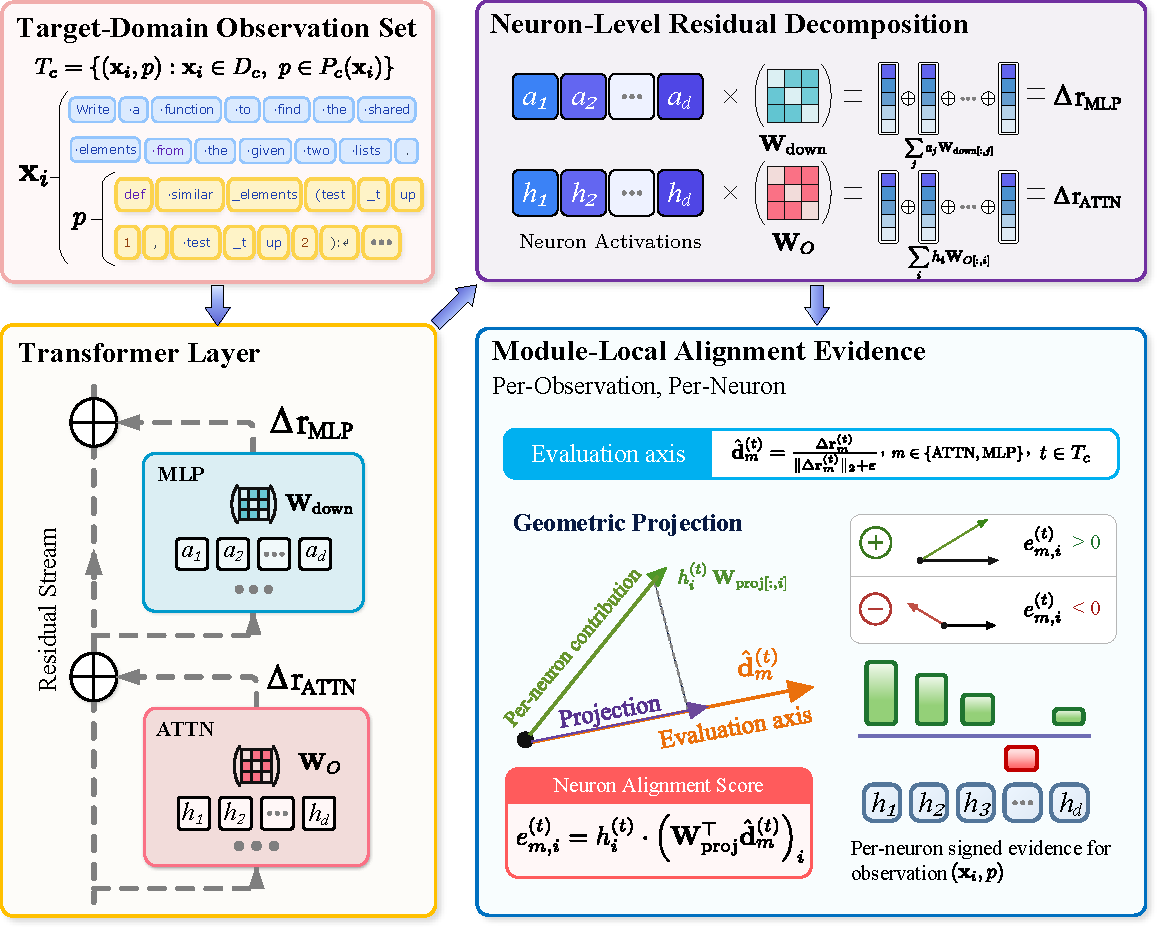
\includegraphics[width=30cm]{assets/race/rda_overview.pdf}\end{center}
\sourcecaption{Original paper, Fig.\ 1: residual-direction alignment (RDA). The axis is the current module's update, and each neuron supplies signed alignment evidence.}
\end{headerbox}
\begin{headerbox}{cam}{col=method2,header={02\quad Estimate, Rank, and Filter},header font=\postersectionfont,
 header style={fill=teal,text=white},body style={fill=white},sep=.65cm,font=\bodyfont}
\textbf{Functional consistency:} positive mean evidence with low variability.
\subhead{Forward-Pass Evidence}
For neuron $j$ at token-position observation $t$:
\[
 e_j^{(t)}=a_j^{(t)}\mathbf w_j^\top\hat{\mathbf d}^{(t)},\qquad
 \hat{\mathbf d}^{(t)}=\frac{\Delta\mathbf r^{(t)}}{\|\Delta\mathbf r^{(t)}\|_2+\varepsilon}.
\]
Here $\mathbf w_j$ is the output-projection column; $a_j$ is the MLP activation or attention output channel.
\subhead{Bayesian Aggregation}
Model $e_j^{(t)}\sim\mathcal N(\mu_j,\sigma_j^2)$ with a Normal-Inverse-Gamma prior. Update from the observation count, mean, and centered sum of squares.
\[
 \mu_j\mid\{e_j^{(t)}\}\sim t_{2\alpha_n}(\mu_{n,j},\sigma_{\mu,j}),\qquad
 \sigma_{\mu,j}^2=\frac{\beta_{n,j}}{\alpha_n\lambda_n}.
\]
\textbf{Conservative Alignment Magnitude (CAM):}
\[
 \mathrm{CAM}_j=\mathbf 1[\mu_{n,j}>0]\max\!\left\{0,\mu_{n,j}-t_{.95,2\alpha_n}\sigma_{\mu,j}\right\}.
\]
The lower credible bound penalizes noisy or scarce evidence. Default prior: $(\mu_0,\lambda_0,\alpha_0,\beta_0)=(0,1,1,1)$; $\gamma=.05$.
\subhead{Reference-Set Filtering (RSF)}
Remove neurons that rank highly on a general reference set (WikiText-2), then retain the top target neurons \textbf{within each layer and module}. Suppress their activations to test behavioral relevance.
\end{headerbox}
\newpostercol{results1}{start={([xshift=2cm,yshift=-63.1cm]poster.north west)},width=39.15cm}
\newpostercol{results2}{start={([xshift=42.95cm,yshift=-63.1cm]poster.north west)},width=39.15cm}
\begin{headerbox}{selectivity}{col=results1,header={03\quad Selective Suppression: Broad to Narrow},header font=\postersectionfont,
 header style={fill=navy,text=white},body style={fill=white},sep=.65cm,font=\bodyfont}
\textbf{Code-selected MLP neurons:} strong target and OOD drops, with much smaller effects on other benchmarks.
\par\vspace{.25cm}
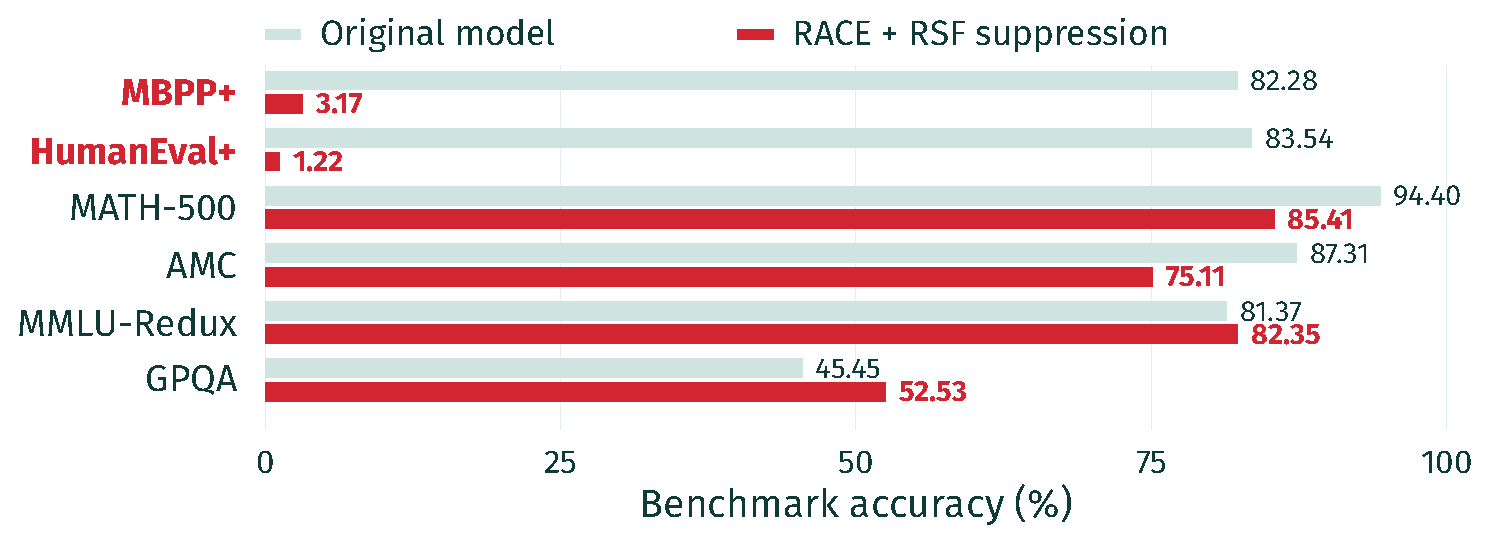
\includegraphics[width=\linewidth]{assets/race/code_accuracy.pdf}\par
\sourcecaption{Qwen3-4B-it; MBPP+ scoring, WikiText-2 RSF, top-1\% MLP suppression per layer. Accuracy averages three runs (Table 21); code targets are orange.}
\vspace{.4cm}
{\centering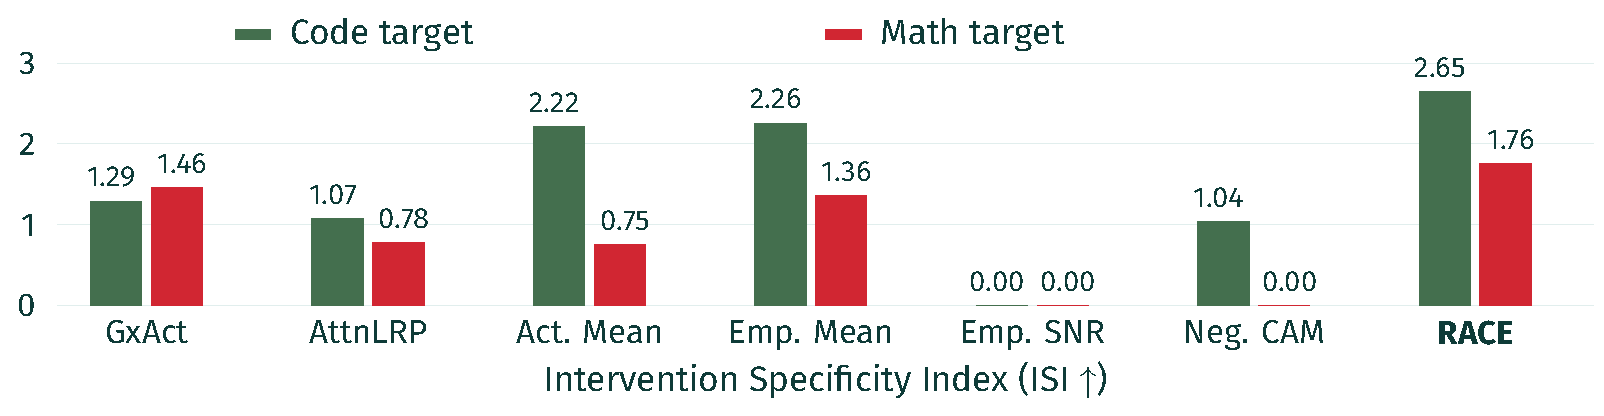
\includegraphics[width=.94\linewidth]{assets/race/isi.pdf}\par}
\sourcecaption{Same top-1\% MLP budget with RSF. ISI measures target drop relative to non-target drop; higher is better (Fig.\ 3; Tables 21, 23).}
\subhead{From Broad Capability to a Narrow Behavior}
{\smallfont\textbf{PyComp-1K:} 1,000 AST-verified Python statements targeting comprehensions. Suppress $K_{\mathrm{sel}}=10$ neurons per layer after RSF.\par}
\vspace{.25cm}
{\centering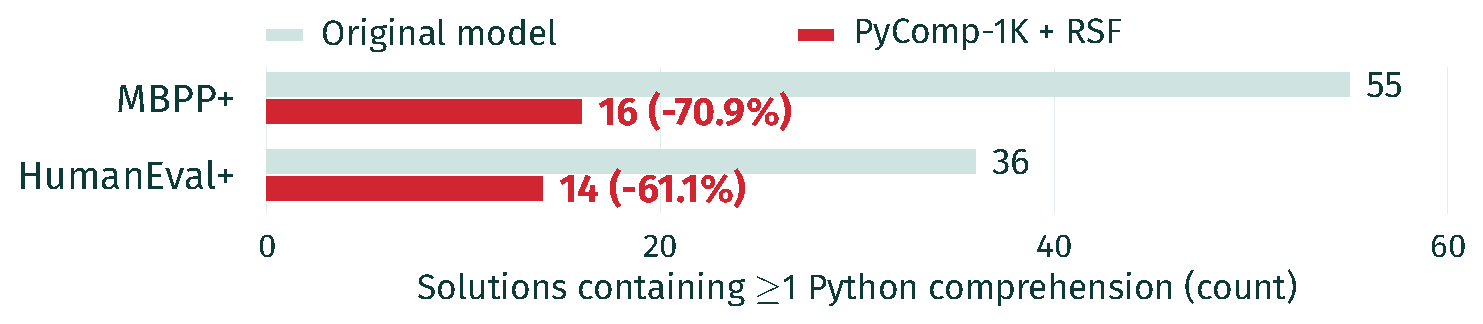
\includegraphics[width=.94\linewidth]{assets/race/comprehensions.pdf}\par}
\sourcecaption{Qwen3-4B-it; number of outputs containing at least one comprehension (Table 5).}
\vspace{.25cm}
{\smallfont Functional correctness on the \textbf{remaining comprehension-using solutions}: MBPP+ 92.73\% $\to$ 87.50\%; HumanEval+ 86.11\% $\to$ 85.71\% (conditional subset scores).\par}
\end{headerbox}
\begin{headerbox}{distribution}{col=results2,header={04\quad Verify the Distributional Effect},header font=\postersectionfont,
 header style={fill=navy,text=white},body style={fill=white},sep=.65cm,font=\bodyfont}
Target-corpus perplexity rises sharply; the general reference corpus changes by less than 3\%.
\par\vspace{.3cm}
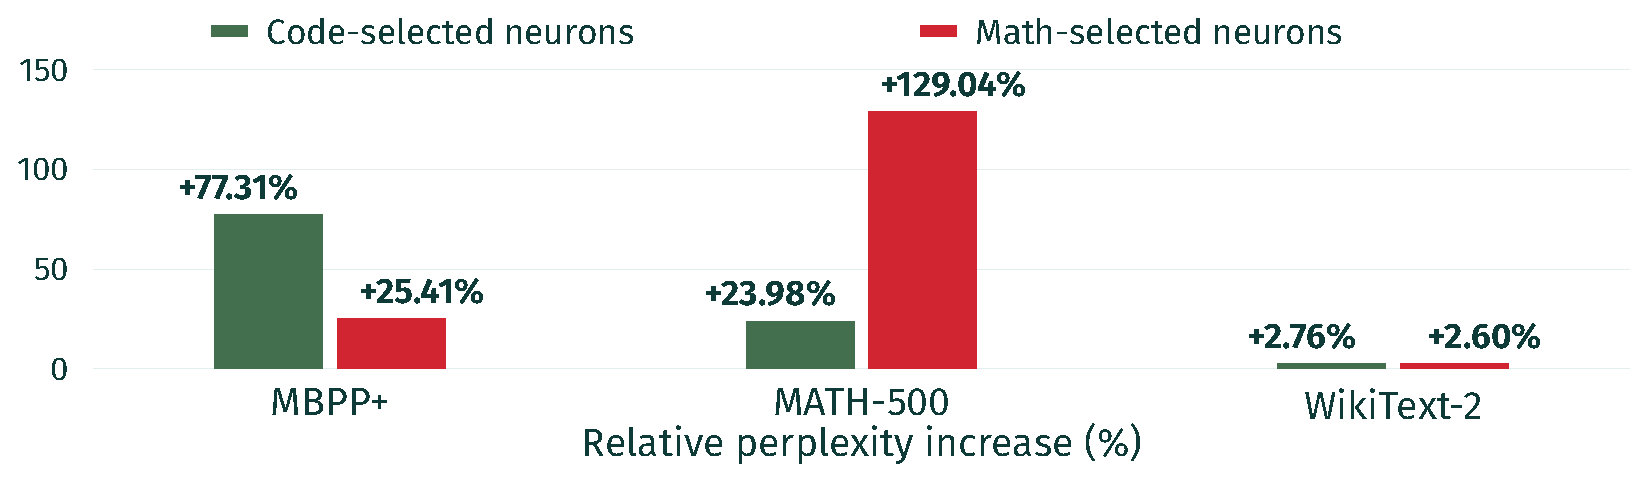
\includegraphics[width=\linewidth]{assets/race/distribution.pdf}\par
\sourcecaption{Qwen3-4B-it, RSF, top-1\% MLP suppression per layer. Relative perplexity increase from Table 4; each color uses its own target scoring set.}
\subhead{The Effect Extends to 32B Models}
{\smallfont OLMo-3.1-32B-it, math scoring + WikiText-2 RSF; top-5\% MLP suppression per layer (Table 3).\par}
\vspace{.3cm}
{\fontsize{29}{37}\selectfont\setlength{\tabcolsep}{.35cm}\renewcommand{\arraystretch}{1.25}
\begin{tabular*}{\linewidth}{@{\extracolsep{0pt plus 1fil}}lrr@{}}
\toprule Benchmark & Original & Suppressed\\\midrule
MATH-500 (target) & 86.40 & \textbf{6.72}\\
AMC (OOD) & 79.85 & \textbf{7.46}\\
GPQA & 48.60 & 37.79\\
MMLU-Redux & 84.70 & 77.79\\\bottomrule
\end{tabular*}\par}
\vspace{.45cm}
{\setlength{\fboxsep}{.45cm}\colorbox{paper}{\parbox{\dimexpr\linewidth-.9cm\relax}{\smallfont\textbf{Scope:} domain-specific effects are stronger in MLPs. Attention channels show greater cross-domain overlap, and RSF yields weaker attention specificity. Linear projections can miss nonlinear interactions.\par}}}
\end{headerbox}
\newpostercol{refcol}{start={([xshift=42.95cm,yshift=-100.3cm]poster.north west)},width=39.15cm}
\begin{headerbox}{refbox}{col=refcol,header={Paper, Code, and Contact},header font=\postersectionfont,
 header style={fill=orange,text=white},body style={fill=white},sep=.65cm,font=\bodyfont}
\begin{center}\qrcode[height=4.2cm]{https://github.com/Nexround/RACE}\end{center}
\vspace{.2cm}
{\smallfont
\textbf{Paper:} arXiv:2608.24758v2\par\vspace{.12cm}
\textbf{Code:} \href{https://github.com/Nexround/RACE}{github.com/Nexround/RACE}\par\vspace{.12cm}
\textbf{Contact:} \href{mailto:2430310032@stmail.ntu.edu.cn}{2430310032@stmail.ntu.edu.cn}\par\vspace{.12cm}
\textsuperscript{*}Corresponding author: \href{mailto:pingpeng@ntu.edu.cn}{pingpeng@ntu.edu.cn}\par}
\end{headerbox}
\newdimen\reportX\newdimen\reportY
\foreach \boxname in {titlebox,leader,rda,cam,selectivity,distribution,refbox} {
\path ($(poster.north)-(\boxname.south)$);\pgfgetlastxy{\reportX}{\reportY}
\typeout{POSTERBOUND \boxname: \reportY}
}
\end{poster}
\end{document}
